%!TEX root = main.tex

\section{Understanding Voice Recognition Performance}
\label{sec:voice}

\begin{table*}[t]
\caption{High-level statistics of voice recognition flows.}
\label{tab:voice_stats}
\centering
\renewcommand{\arraystretch}{1.0}
\begin{tabular}{c|c|c|c|C{2.1cm}|C{2.1cm}}
	\hline
	& finish time (sec.) & flow size (\#pkts) & RTT (ms) & \% of flows w/ disord. pkts & \% of flows w/ timeout retx \\
	\hline
	WiFi & 0.069 (0.015, 1.052) & 3.0 (2.0, 4.0) & 45 (12, 399) & 3.3\% & 9.5\% \\
	%\hline
	3G & 0.055 (0.006, 0.316) & 3.0 (2.0, 4.0) & 35 (5, 99) & 6.6\% & 7.3\% \\
	\hline
\end{tabular}
\end{table*}

%\begin{figure}[th]
%	\centering
%	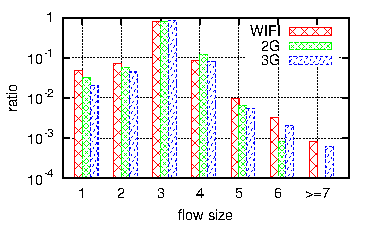
\includegraphics[width=0.8\linewidth]{voice_flow_size}
%	\caption{The number of voice data packets in voice recognition flows.}
%	\label{fig:voice_flow_size}
%\end{figure}





We look at the TCP performance of voice recognition flows in this section. We first provide a high-level statistics on the key performance factors for 3G and WiFi flows in Table \ref{tab:voice_stats}. For finish time, flow size and RTT, we report the median along with the $5th$ percentile and $95th$ percentile values in the parenthesis. The flow size measures the number of voice data packets. Independent of the access type, nearly all voice recognition flows contains no more 4 voice data packets. Given that the initial congestion window in current Android TCP/IP stack is set to 10 segments\cite{dukkipati2010argument}, the voice data can be transmitted in the initial congestion window. Another interesting observation from Table \ref{tab:voice_stats} is that 3G flows tend to have smaller RTTs but a higher probability of suffering from packet disordering. In what follows, we examine each TCP performance factor and its impact on the finish time in detail. 

\subsection{RTT Analysis}

As illustrated in Figure~\ref{fig:voice_estimate_rtt}, we can measure at most 3 RTTs at server side in a voice recognition flow. However, RTT is ambiguous when the corresponding segments for RTT measures are retransmitted. To tackle this problem, we use the following methodology to determine the \emph{minimal RTT}. If no retransmission happens for SYN packets, $t^s_a - t^s_s$ is used as the RTT of the flow, i.e. the RTT is measured during 3WHS (3-way handshake). Otherwise, the RTT measured during connection termination is preferred if the FIN packet is not retransmitted. In the case that both of the above RTTs are ambiguous, $t^s_t - t^s_r$ is used as the measured RTT. We have verified using our datasets that the RTT measured during 3WHS is the minimal RTT in more than 60\% of flows, and is less than 2 times of the minimal RTT in 95\% of flows. Thus it is reasonable to assume that the RTT measured using the above methodology is close to the minimal RTT of the flow.



Figure~\ref{fig:voice_rtt} plots the distribution of RTTs measured in individual voice recognition flows. The median RTT of 3G flows is around 35 ms. WiFi flows on the other hand exhibit a higher RTT with a median around 45 ms. In particular, while 95\% of 3G flows have a RTT less than 100 ms, as many as 20\% of WiFi flows have a RTT larger than this value. 

\begin{figure}[th]
\centering
	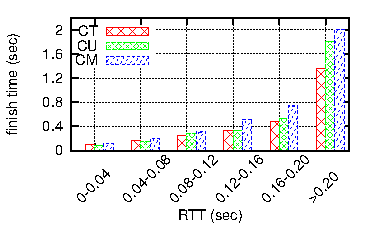
\includegraphics[width=0.8\linewidth]{voice_rtt}
\caption{Distribution of RTTs in voice recognition flows.}
\label{fig:voice_rtt}
\end{figure}

\begin{figure}[th]
\centering
	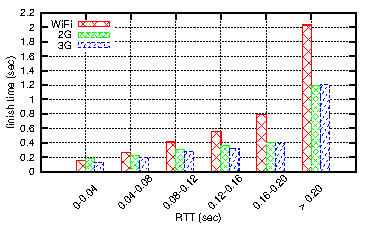
\includegraphics[width=0.8\linewidth]{voice_rtt_finish_time}
\caption{Impact of RTT on finish time for voice recognition flows.}
\label{fig:v_rtt_time}
\end{figure}

RTT is a major factor that affects TCP performance. We further examine the impact of RTT on flow finish time in Figure \ref{fig:v_rtt_time}. We observe that for flows with RTT no larger than 200 ms, the finish time increases in proportional to the RTT: the ratio of finish time to RTT is about 2.5 for 3G flows and about 4 for WiFi flows. Since the finish time of a voice cognition is approximately $2RTT$ plus the time for voice data uploading, the difference of the ratio between cellular network and WiFi network should come from the time for data uploading. One possibility is that the RTT during data transferring in WiFi network is significantly larger than the RTT measured during connection establishment (i.e. 3WHS) \cite{UM-CS-2012-022}, where we obtained most of the RTTs. It seems that 3G networks provide similar performance in terms of RTT during 3WHS and data transferring. 

The finish time becomes extremely large when RTT is beyond 0.2 second. Such a large RTT is an indication of network congestion as in TCP Vegas\cite{brakmo1995tcp} and FastTCP\cite{wei2006fast}. In other words, it is likely that the flow is traversing congested network and may encounter packet loss, which may take a relatively long time for recovery.

\subsection{Packet Disordering Analysis}
\label{sec:v_pd}


\begin{figure*}[th]
\centering
	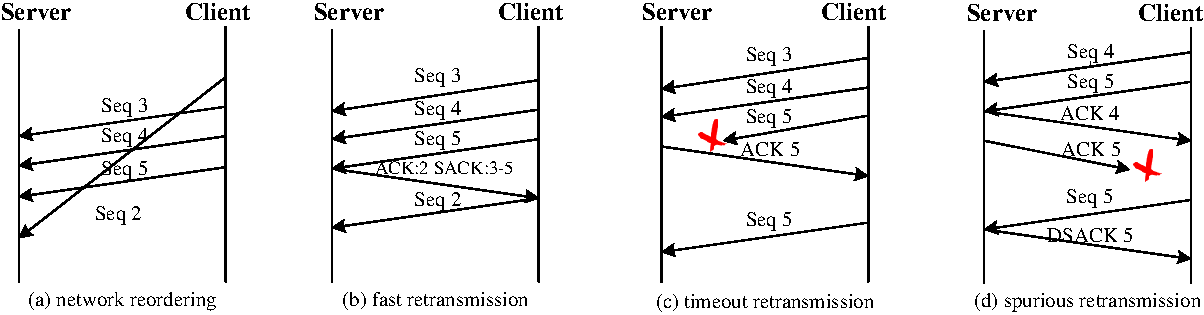
\includegraphics[scale=0.7]{voice_flow_estimate_retrans}
\caption{Server could not distinguish packet reordering events, which are (a) network reordering, (b) fast retransmit, and (c) timeout retransmission. Server may identify some timeout retransmissions as long packet delay (d).}
\label{fig:voice_flow_estimate_retrans}
\end{figure*}

Another factor that could heavily impact the finish time is the network congestion events, which can be observed by servers as packet loss, packet delay and packet reordering. However, as a TCP receiver, the server might not be able to identify the exact network congestion event type. For example, the server observes the same packet sequences for Figure~\ref{fig:voice_flow_estimate_retrans}(a), \ref{fig:voice_flow_estimate_retrans}(b) and \ref{fig:voice_flow_estimate_retrans}(c), despite that they depict 3 types of congestion: packet reordering in Figure~\ref{fig:voice_flow_estimate_retrans}(a), fast retransmit for packet loss recovery in Figure~\ref{fig:voice_flow_estimate_retrans}(b) and timeout retransmission for packet loss recovery in Figure~\ref{fig:voice_flow_estimate_retrans}(c). These observations imply the difficulty of performing TCP analysis at server side for uploading sessions. 



We thus directly use the number of disordered packets, a metric that server can accurately obtain, to capture the network congestion characteristics. In the examples shown in the first 3 subfigures in Figure~\ref{fig:voice_flow_estimate_retrans}, the number of disordered packets is 1. %As we have shown in Figure~\ref{fig:voice_flow_estimate_retrans}, a disordered packet seen by the serve could be caused by either packet reordering, fast retransmit or timeout retransmission for packet loss recovery (i.e. Figure~\ref{fig:voice_flow_estimate_retrans}(a-c)). 
We report the percentage of flows with packet disordering in Table~\ref{tab:voice_reorder}.

%\begin{table}[th]
%\caption{Distribution of the number of disordered packets.}
%\label{tab:voice_reorder}
%\centering
%\renewcommand{\arraystretch}{1.1}
%\begin{tabular}{c|c|c|c}
%\toprule
%\# disord. pkts & WiFi & 2G & 3G \\
%\hline
%0 & 96.7\% & 94.4\% & 93.3\% \\
%%\hline
%1 & 3.03\% & 5.5\% & 6.6\% \\
%%\hline
%%2 & 0.1\% & - & - \\
%%\hline
%$\ge$2 & 0.2\% & - & - \\
%\bottomrule
%\end{tabular}
%\end{table}

\begin{table}[th]
\caption{Percentage of flows with packet disordering.}
\label{tab:voice_reorder}
\centering
\renewcommand{\arraystretch}{1.0}
\begin{tabular}{c|c|c|c}
	\hline
	\# disord. pkts & 0 & 1 & $\ge$2 \\
	\hline
	WiFi & 96.7\% & 3.03\% & 0.2\% \\
	\hline
	3G & 93.3\% & 6.6\% & - \\
	\hline
\end{tabular}
\end{table}

As expected, the majority of flows experience no packet disordering. But we did observe that 6.6\% of 3G flows and 3\% of WiFi flows have one disordered packet. The fraction of flows having more than 2 disordered flows is negligible. Given that in most cases, the voice data only consists of 3 packets, even one disordered packet could severely impair the uploading performance as shown in Figure \ref{fig:voice_reorder}.


\begin{figure}[th]
\centering
	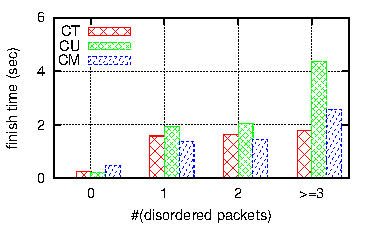
\includegraphics[width=0.8\linewidth]{voice_reorder}
\caption{Impact of packet disordering on finish time.}
\label{fig:voice_reorder}
\end{figure}

We can see from Figure \ref{fig:voice_reorder} that one disordered packet in 3G uploading flows can increase the median finish time from 10 ms to 60 ms, while for WiFi flows we even observe as many as 20\% of those suffering from packet disordering cannot finish the uploading within 1 second. When receiving a disordered packet, the server feeds back to the client with an SACK (as shown in Figure~\ref{fig:voice_flow_estimate_retrans}). The client will retransmit the packet in the hole (\ie the disordered packet) after collecting 3 SACKs. In the case that not sufficient number of SACKs can be collected, the client has to rely on the expensive timeout retransmission for recovery. %That said, the increased finish time might be caused by either packet delay, fast retransmit or timeout retransmission. Unfortunately, we cannot identify how much each of these congestion events contributes using the datasets collected from server side.

The significance of the impact of packet disordering on finish time is also dependent on RTT, because both the waiting time for fast retransmit and timeout retransmission timer (\ie RTO) depend on the RTT. To further assess the objective impact of packet reordering by excluding the possible effect of other covariates (like RTT), we implement a non-parametric factorial analysis framework using a Quasi Experimental Design (QED) \cite{krishnan2013video}. In QED, each uniformly sampled individual $u$ is compared with an individual $v$ randomly selected from those that have identical covariates with $u$ but the cause variable (packet disordering in our context). And thus, any outcome difference between these two individuals can be attributed to the cause variable we are tracking. 

In detail, we bin for each access type the voice recognition flows into two groups: those with no disordered packet ($G_1$) and those with 1 disordered packet ($G_2$). For each flow $u \in G_1$, we randomly choose a flow $v$ from $G_2$ that has similar RTT (i.e. the difference is less than 40 ms) and and the same condition whether encountering a timeout retransmission that is identified by the methodology in Section \ref{sec:v_rto}. We record the outcome difference as $o_{u,v} = \frac{ftime_{v} - ftime_{u}}{ftime_{u}}$, where $ftime_v$ is the finisht time of the flow $v$. Finally, we average all the outcome differences over the matched pairs and use this average difference to gauge the impact of packet disordering.

\begin{table}[th]
\caption{QED results for the impact of packet disordering.}
\label{tab:voice_qed_reorder}
\centering
\renewcommand{\arraystretch}{1}
\begin{tabular}{C{1cm}|C{1.5cm}|C{1.5cm}}
	\hline
	 & WiFi & 3G \\
	\hline
	QED & 6.42 & 4.45 \\
	\hline
\end{tabular}
\end{table}

Table~\ref{tab:voice_qed_reorder} presents the QED results, which show that one disordered packet can lead to an increase of finish time by as large as $4-6$ times. The larger finish time increase of WiFi flows than 3G flows is possibly because the packet disordering events in WiFi flows are more likely to be caused by packet losses (i.e. Figure \ref{fig:voice_flow_estimate_retrans}(b) and \ref{fig:voice_flow_estimate_retrans}(c)), which require to using more time to recovery. Indeed, we find using the web search dataset that the packet loss rate in WiFi is 3.9\% and is 0.9\% in 3G\footnote{We cannot obtain the packet loss rate of voice recognition flows as the server where we collected our dataset is a TCP receiver}. 

\subsection{Timeout Retransmission Analysis}\label{sec:v_rto}

\begin{figure}[th]
\centering
	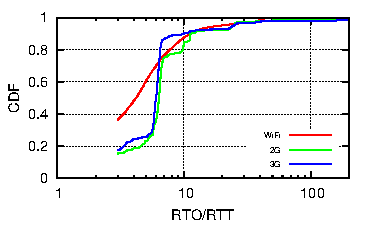
\includegraphics[width=0.8\linewidth]{voice_rtt_rto_ratio}
\caption{Distribution of RTO/RTT}
\label{fig:rto_rtt}
\end{figure}

We rely on the time gap between actual arrival time and the estimated arrival time of individual packets to infer timeout retransmissions in voice recognition flows that show the similar behavior in in Figure \ref{fig:voice_flow_estimate_retrans}(d). The estimated arrival time of a packet is the mean value of the arrival time of its preceding packet and subsequent packets. In the case that this gap is larger than RTO, the transmission of the packet is identified as a timeout retransmission. However, the server does not know the client-side RTO. We thus have to estimate the RTO. RTO in TCP implementation is set to $\text{SRTT} + max(200ms, 4 \text{ RTTVAR})$\cite{rfc62982011computing}, where SRTT is close to RTT, and RTTVAR is approximately $RTT/2$, i.e. $\widehat{RTO} \approx RTT + max(200ms, 2 RTT)$. It is noteworthy that the timeout retransmissions identified using the above methodology are not overlapped with the those shown in Figure \ref{fig:voice_flow_estimate_retrans}(c).


We first examine how large RTOs can be in Figure \ref{fig:rto_rtt}, where we plot the distribution of RTO/RTT. We can observe the median RTO is around several time of RTT, but can be as large as tens of or hundreds of RTT. Given that a time retransmission takes a RTO for recovery, the impact of timeout retransmission on flow finish time can be extremely large.

\begin{table}[th]
\centering
\renewcommand{\arraystretch}{1.1}
\caption{Flows with timeout retransmission.}
\label{tab:voice_timeout_stats}
\begin{tabular}{c | C{2cm} | C{2cm}}
	\hline
	 & WiFi & 3G \\
	\hline
	% packet reordering & 3.2\% & 5.6\% & 6.2\% \\
	% \hline
	3WHS retx & 2.6\% & 0.8\% \\
	%\hline
	data retx & 9.5\%  & 7.3\% \\
	% \hline
	% incomplete transmission & 0.2\% & 0.3\% & 2.4\% \\
	\hline
\end{tabular}
\end{table}

Table~\ref{tab:voice_timeout_stats} lists the percentage of flows that suffer from at least one timeout retransmission in our dataset. The timeout retransmission could happen either during 3-way handshake (3WHS) or in data transmission. While the timeout retransmission during 3WHS is less likely to happen compared with timeout retransmission during data uploading, its impact might be even larger. This is because the initial RTO is set to 1 second \cite{rfc62982011computing} as there is no RTT available at that time. This RTO value is often much larger than that computed during data uploading. Users might quit the app during this the time period for recovery. In addition, a timeout retransmission during 3WHS result in the congestion window size to 1, which further impair the performance for data transmission.

Regardless of the access type, we observe as many as over 7\% of the voice data uploading flows suffer from at least one timeout retransmission. Such a large fraction of timeout retransmission flows can be explained by the fact that almost all the voice recognition flows contain no more than 4 voice data packets. When one of the last three packets is dropped, the sender (i.e. client) has to rely on RTO for retransmission. This behavior is similar to the tail lost one identified in \cite{flach2013reducing}. But in the voice data uploading context, the server is no longer a sender and thus unable to eliminate such kind of RTO retransmissions by gently send redundant packets as proposed in \cite{flach2013reducing}. Our results highlight the necessary of TCP optimization for uploading at server side. 

\begin{figure}[th]
\centering
	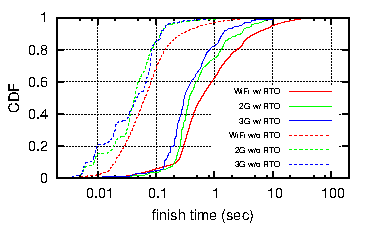
\includegraphics[width=0.8\linewidth]{voice_timeout}
\caption{CDF of finish time of flows with and without RTO.}
\label{fig:voice_rto}
\end{figure}

We finally compare the finish time between flows with and without timeout retransmission in Figure~\ref{fig:voice_rto}, where the $x$-axis is in log scale. The timeout retransmission increases the median finish time from 64 ms to 595 ms.  This is not surprising given that RTO is several times of the RTT. Perhaps more importantly, we observe 10\% of WiFi flows with timeout retransmissions require to using as many as 5 seconds to upload the voice data. The voice search sessions that correspond to these flows are indeed likely to be terminated. In fact, since the number of voice data packets is relatively small ($\le 4$), which can be uploaded within $2\times RTTs$, the time retransmission time (i.e. RTO) will dominate the finish time of those flows that experience timeout retransmissions.  Overall, a larger fraction of WiFi flows suffer from timeout retransmission compared with 3G flows, which partially explains the larger finish time observed in Figure \ref{fig:voice_finish_time}.

\subsection{Summary of Voice Recognition Analysis}

The key observations on voice recognition flows are summarized as follows.
\begin{itemize}
	\item 95\% of voice recognition flows contain no more than 4 data packets, which could be fitted into the initial congestion window from client. Thus ideally the voice data could be transmitted in 1 RTT.
	\item For flows with smaller RTT (less than 200ms in WiFi), the finish time is proportional to the RTT value. However, flows with larger RTT (more than 200ms) experience intolerably long finish time. Flows in WiFi network experience longer finish times than those in cellular network, because of larger RTT.
	\item Disordered packet, as an indication of packet loss, requires time for loss recovery, increasing finish time by 4-6 times. Even though WiFi flows have less number of disordered packets than 3G flows, they suffer more from the disordered packets.
	\item WiFi flows suffer more timeout retransmissions that 3G flows. Those flows experience timeout retransmission either in establishing connections (2.6\%) or in data transfer (9.5\%). Flows with timeout retransmission have finish time one order of magnitude larger than those without timeout retransmission.
\end{itemize}
